% TODO: Teilaufgaben Klausur

\documentclass{beamer}

\usetheme{metropolis}

\usepackage[ngerman]{babel}
\usepackage[autostyle=true,german=quotes]{csquotes}
\usepackage[linewidth=1pt]{mdframed}
\usepackage{hyperref}
\usepackage{makecell}
\usepackage{pifont}
\usepackage{tikz}
\usetikzlibrary{positioning, calc, arrows, fit, decorations.pathreplacing, shapes, shapes.multipart, snakes, trees, automata}
\usepackage{verbatim}
\usepackage{textcomp}
\usepackage{centernot}
\usepackage{tabularx}
\usepackage[normalem]{ulem}
\usepackage{mathpartir}
\usepackage{pdfpages}
\usepackage{wasysym}
\usepackage{qtree}
\usepackage{pgfplots}

\batchmode

\hypersetup{
	colorlinks,
	urlcolor=blue,
	linkcolor=black % for ToC
}
\newenvironment{qaa}[1]{
	#1

	\begin{mdframed}
		\small
}{
	\end{mdframed}
}

\newcommand{\true}{\ding{51}}
\newcommand{\false}{\ding{55}}
\newcommand{\code}[1]{
	\begin{mdframed}
		\verbatiminput{#1}
	\end{mdframed}
}

% lambda calculus stuff

\newcommand{\app}[2]{#1\;#2}
\newcommand{\appr}[2]{\app{\uline{#1}}{\uwave{#2}}}
\newcommand{\lam}[2]{\lambda #1.\, #2}
\newcommand{\appp}[3]{\app{\app{#1}{#2}}{#3}}
\newcommand{\apppp}[4]{\app{\app{\app{#1}{#2}}{#3}}{#4}}
\newcommand{\apppr}[3]{\app{\appr{#1}{#2}}{#3}}

\newcommand{\lamlet}[3]{\texttt{let} \;\; #1 = #2 \;\; \texttt{in} \;\; #3}

\newcommand{\ctrue}{c_\text{true}}
\newcommand{\cfalse}{c_\text{false}}
\newcommand{\cand}{\text{AND}}

\newcommand{\csucc}{\text{succ}}
\newcommand{\cn}[1]{c_{#1}}

\newcommand{\cpair}{\text{pair}}
\newcommand{\cfst}{\text{fst}}
\newcommand{\csnd}{\text{snd}}
\newcommand{\ccurry}{\text{curry}}
\newcommand{\cuncurry}{\text{uncurry}}

\newcommand{\cnil}{\text{nil}}
\newcommand{\ccons}{\text{cons}}
\newcommand{\chead}{\text{head}}
\newcommand{\ctail}{\text{tail}}
\newcommand{\creplicate}{\text{replicate}}

\newcommand{\subst}[3]{(#1)\left[#2\,\to\,#3\right]}

% unification etc.

\newcommand{\functor}[2]{\texttt{#1}(#2)}
\newcommand{\pa}[1]{\texttt{#1}}
\newcommand{\plsunify}{\stackrel{!}{=}}
\newcommand{\unifier}[1]{\left[#1\right]}
\newcommand{\su}[2]{#1 \; \text{\pointer} \; #2}


\title{Tutorium 08: Typisierung \& Typinferenz}
% \subtitle{}
\author{Paul Brinkmeier}
\institute{Tutorium Programmierparadigmen am KIT}
\date{20. Dezember 2022}

\begin{document}

\begin{frame}
    \titlepage
\end{frame}

\section{Typisierung}

{
\setbeamercolor{background canvas}{bg=}
\includepdf{robinson2.pdf}
}

\subsection{Klausuraufgabe WS16/17 A3 a)}

\begin{frame}{Klausuraufgabe WS16/17 A3 a) (6P.)}
  \begin{align*}
    C_1 &= \{ \alpha_9 = \alpha_{10} \to \alpha_8, \alpha_9 = \alpha_4, \alpha_{10} = \texttt{bool} \} \\
    C_2 &= \{ \alpha_{12} = \alpha_{13} \to \alpha_{11}, \alpha_{12} = \alpha_4, \alpha_{13} = \texttt{int} \}
  \end{align*}

  \only<1>{
  \footnotesize
  \begin{enumerate}[i.]
    \item Geben Sie allgemeinste Unifikatoren $\sigma_1$ für $C_1$ und $\sigma_2$ für $C_2$ an.
    \item Ist auch $C_1 \cup C_2$ unifizierbar?
    \item Ist der Ausdruck\\
      \begin{equation*}\lam{a}{\lam{f}{\app{\app{\var{f}}{(\app{\var{a}}{true})}}{(\app{\var{a}}{17})}}}\end{equation*}\\
        typisierbar? Begründen Sie ihre Antwort \emph{kurz}.
  \end{enumerate}
  }

  \only<2>{
    Geben Sie allgemeinste Unifikatoren $\sigma_1$ für $C_1$ und $\sigma_2$ für $C_2$ an.

    \begin{align*}
      \sigma_1 &= \texttt{unify}(\{ \alpha_9 = \alpha_{10} \to \alpha_8, \alpha_9 = \alpha_4, \alpha_{10} = \texttt{bool} \}) \\
               &= ... = \unifier{\su{\alpha_9}{\pa{bool} \to \alpha_8}, \su{\alpha_4}{\pa{bool} \to \alpha_8}, \su{\alpha_{10}}{\pa{bool}}} \\
      \sigma_2 &= \texttt{unify}(\{ \alpha_{12} = \alpha_{13} \to \alpha_{11}, \alpha_{12} = \alpha_4, \alpha_{13} = \texttt{int} \}) \\
               &= ... = \unifier{\su{\alpha_{12}}{\pa{int} \to \alpha_{11}}, \su{\alpha_4}{\pa{int} \to \alpha_{11}}, \su{\alpha_{13}}{\pa{int}}}
    \end{align*}
  }

  \only<3>{
    Ist auch $C_1 \cup C_2$ unifizierbar?
    \begin{align*}
      \sigma_1 &= ... = \unifier{\su{\alpha_9}{\pa{bool} \to \alpha_8}, \underline{\su{\alpha_4}{\pa{bool} \to \alpha_8}}, \su{\alpha_{10}}{\pa{bool}}} \\
      \sigma_2 &= ... = \unifier{\su{\alpha_{12}}{\pa{int} \to \alpha_{11}}, \underline{\su{\alpha_4}{\pa{int} \to \alpha_{11}}}, \su{\alpha_{13}}{\pa{int}}}
    \end{align*}

    A: Nein, da die \emph{allgemeinsten Unifikatoren} $\sigma_1$ und $\sigma_2$ einen Konflikt für $\alpha_4$ enthalten:
    $\texttt{unify}(\{ \pa{bool} = \pa{int} \}) = \texttt{fail}$
  }

  \only<4>{
    Ist der Ausdruck\\
      \begin{equation*}\lam{a}{\lam{f}{\app{\app{\var{f}}{(\app{\var{a}}{true})}}{(\app{\var{a}}{17})}}}\end{equation*}\\
    typisierbar? Begründen Sie ihre Antwort \emph{kurz}.

    \vfill

    A: Nein, da $\var{a}$ mit zwei verschiedenen Typen verwendet wird.
  }
\end{frame}

\newcommand{\tikzmark}[3]{\tikz[baseline, remember picture]{
	\node[fill=#1,draw] (#2) {#3};
}}

\begin{frame}{Cheatsheet: Typisierter Lambda-Kalkül}
  \begin{mathpar}
    \inferrule{
      \Gamma{}, \var{p} : \pi \vdash b : \rho
    }{
      \Gamma \vdash \lam{p}{b} : \pi \to \rho
    } \textrm{\textsc{Abs}}
    \and
    \inferrule{
      \Gamma \vdash f : \phi \to \alpha \\
      \Gamma \vdash x : \phi
    }{
      \Gamma \vdash \app{f}{x} : \alpha
    } \textrm{\textsc{App}}
    \and
    \inferrule{
      \Gamma{}(\var{t}) = \tau
    }{
      \Gamma \vdash \var{t} : \tau
    } \textrm{\textsc{Var}}
    \and
    \inferrule{
      c \in \textsc{Const}
    }{
      \Gamma \vdash c : \tau_c
    } \textrm{\textsc{Const}}
  \end{mathpar}

  \begin{itemize}
    \item Typvariablen: $\tau$, $\alpha$, $\pi$, $\rho$
    \item Funktionstypen: $\tau_1 \to \tau_2$, rechtsassoziativ
    \item \emph{Typisierungsregeln sind eindeutig}: Eine Regel pro Termform
  \end{itemize}
\end{frame}

\begin{frame}{Was bedeuten eigentlich $\vdash$, $\Gamma$ und $:$?}
  \begin{equation*}
    \lam{a}{\lam{f}{\app{\var{f}}{(\app{\var{a}}{true})}}}
  \end{equation*}

  Um zu einem solchen Term ein Typisierungsproblem zu beschreiben, notieren wir:

  \begin{equation*}
    \Gamma \vdash \lam{a}{\lam{f}{\app{\var{f}}{(\app{\var{a}}{true})}}} : \tau
  \end{equation*}

  \enquote{Im \emph{Typkontext} $\Gamma$ hat der Term den Typen $\tau$.}

  \begin{itemize}
    \item $\Gamma$: Enthält Typen für freie Variablen.
    \item Liste von Paaren aus Variablen und deren Typen
    \item Liste $\leadsto$ Reihenfolge ist wichtig
  \end{itemize}
\end{frame}

\begin{frame}{$\Gamma$ in Aktion}
  \begin{align*}
    &\Gamma \vdash \var{a} + 42 : \pa{int} \\
    &\textsc{Const} = \{ 42 \}, \tau_{42} = \texttt{int}
  \end{align*}

  Damit die Aussage \enquote{$\var{a} + 42$ hat in $\Gamma$ den Typen \texttt{int}} stimmt, müssen wir für $\Gamma$ wählen:
  
  \begin{itemize}
    \pause
    \item $\Gamma = \var{a} : \texttt{int}, + : \texttt{int} \to \texttt{int} \to \texttt{int}$
    \pause
    \item Allgemeiner: $\Gamma = \var{a} : \alpha, + : \alpha \to \texttt{int} \to \texttt{int}$
  \end{itemize}
\end{frame}

\subsection{Typisierungsregeln im Detail}

\begin{frame}{Typisierungsregel für Lambdas}
	\begin{itemize}
		\item \tikzmark{green!20}{contextL}{\enquote{Unter Einfügung des Typs $\pi$ von $\var{p}$ in den Kontext...}}
		\item \tikzmark{red!20}{bodyTypeL}{\enquote{... ist $b$ als Funktion von $\var{p}$ typisierbar.}}
	\end{itemize}

	\begin{mathpar}
		\inferrule{
			\tikzmark{green!20}{context}{$\Gamma{}, p : \pi$} \\
			\tikzmark{red!20}{bodyType}{$\vdash b : \rho$}
		}{
			\tikzmark{blue!20}{absType}{$\Gamma \vdash \lam{p}{b} : \pi \to \rho$}
                } \textrm{\textsc{Abs}}
	\end{mathpar}

	\begin{itemize}
		\item Daraus folgt:
		\item \tikzmark{blue!20}{absTypeL}{\enquote{$\lam{p}{b}$ ist eine Funktion, die $\pi$s auf $\rho$s abbildet}}
	\end{itemize}

	\tikz[overlay, remember picture]{
		\draw[->] (bodyTypeL) edge [bend left] (bodyType);
		\draw[->] (contextL) edge [bend right] (context);
		\draw[->] (absTypeL) edge [bend left] (absType);
	}
\end{frame}

\begin{frame}{Typisierungsregel für Funktionsanwendungen}
	\begin{itemize}
		\item \tikzmark{green!20}{fTypeL}{\enquote{$f$ ist im Kontext $\Gamma$ eine Funktion, die $\phi$s auf $\alpha$s abbildet.}}
		\item \tikzmark{red!20}{aTypeL}{\enquote{$x$ ist im Kontext $\Gamma$ ein Term des Typs $\phi$.}}
	\end{itemize}
	\begin{mathpar}
		\inferrule{
			\tikzmark{green!20}{fType}{$\Gamma \vdash f : \phi \to \alpha$} \\
			\tikzmark{red!20}{aType}{$\Gamma \vdash x : \phi$}
		}{
			\tikzmark{blue!20}{eType}{$\Gamma \vdash \app{f}{x} : \alpha$}
                } \textrm{\textsc{App}}
	\end{mathpar}

	\begin{itemize}
		\item Daraus folgt:
		\item \tikzmark{blue!20}{eTypeL}{\enquote{$x$ eingesetzt in $f$ ergibt einen Term des Typs $\alpha$.}}
	\end{itemize}

	\tikz[overlay, remember picture]{
		\draw[->] (fTypeL) edge [bend right] (fType);
		\draw[->] (aTypeL) edge [bend left] (aType);
		\draw[->] (eTypeL) edge [bend left] (eType);
	}
\end{frame}

\begin{frame}{Einfache Typisierungsregel für Variablen}
	\begin{itemize}
		\item \tikz[baseline, remember picture]{\node [fill=green!20,draw] (varRetL) {\enquote{Der Typkontext $\Gamma$ enthält einen Typ $\tau$ für $\var{t}$.}};}
	\end{itemize}

	\begin{mathpar}
		\inferrule{
			\tikz[baseline, remember picture]{\node[fill=green!20,draw] (varRet) {$\Gamma{}(\var{t}) = \tau$};}
		}{
			\tikz[baseline, remember picture]{\node[fill=blue!20,draw] (varShow) {
				$\Gamma \vdash \var{t} : \tau$
			};}
		} \textrm{\textsc{Var}}
	\end{mathpar}

	\begin{itemize}
		\item Daraus folgt:
		\item \tikz[baseline, remember picture]{\node [fill=blue!20,draw] (varShowL) {\enquote{Variable $\var{t}$ hat im Kontext $\Gamma$ den Typ $\tau$.}};}
	\end{itemize}

	\tikz[overlay, remember picture]{
		\draw[->] (varShowL) edge [bend left] (varShow);
		\draw[->] (varRetL) edge [bend right] (varRet);
	}
\end{frame}

% https://tex.stackexchange.com/questions/9466/color-underline-a-formula
\def\mathunderline#1#2{\color{#1}\underline{{\color{black}#2}}\color{black}}

\begin{frame}{Typisierung: Beispiel}
  \only<1>{
    \begin{mathpar}
      \var{x} : \texttt{bool} \vdash \lam{f}{\app{\var{f}}{\var{x}}} : (\texttt{bool} \to \alpha) \to \alpha
    \end{mathpar}

    \enquote{Unter der Annahme, dass $\var{x}$ den Typ \texttt{bool} hat, hat $\lam{f}{\app{\var{f}}{\var{x}}}$ den Typ $(\texttt{bool} \to \alpha) \to \alpha$.}
  }

  \only<2>{
    \begin{mathpar}
      \inferrule{
        \mathunderline{red}{\var{x} : \texttt{bool}}, \mathunderline{blue}{\var{f}} : \mathunderline{yellow}{\texttt{bool} \to \alpha} \vdash
        \mathunderline{green}{\app{\var{f}}{\var{x}}} :
        \mathunderline{orange}{\alpha}
      }{
        \mathunderline{red}{\var{x} : \texttt{bool}} \vdash \lam{\mathunderline{blue}{\var{f}}}{\mathunderline{green}{\app{\var{f}}{\var{x}}}} : (\mathunderline{yellow}{\texttt{bool} \to \alpha}) \to \mathunderline{orange}{\alpha}
      } \textsc{Abs}
    \end{mathpar}

    \enquote{Pattern-Matching}: Der äußerste Term ist ein Lambda, also wenden wir die $\textsc{Abs}$-Regel an.

    \begin{columns}
        \begin{column}{0.5\textwidth}
    \begin{align*}
      \mathunderline{red}{\Gamma} &= \mathunderline{red}{\var{x} : \texttt{bool}} \\
      \mathunderline{blue}{p} &= \mathunderline{blue}{\var{f}}, \mathunderline{green}{\var{b}} = \mathunderline{green}{\app{\var{f}}{\var{x}}} \\
      \mathunderline{yellow}{\pi} &= \mathunderline{yellow}{\texttt{bool} \to \alpha} \\
      \mathunderline{orange}{\rho} &= \mathunderline{orange}{\alpha}
    \end{align*}
\end{column}
\begin{column}{0.5\textwidth}

    \begin{mathpar}
      \inferrule{
        \mathunderline{red}{\Gamma{}}, \mathunderline{blue}{\var{p}} : \mathunderline{yellow}{\pi} \vdash \mathunderline{green}{b} : \mathunderline{orange}{\rho}
      }{
        \mathunderline{red}{\Gamma} \vdash \lam{\mathunderline{blue}{p}}{\mathunderline{green}{b}} : \mathunderline{yellow}{\pi} \to \mathunderline{orange}{\rho}
      } \textrm{\textsc{Abs}}
    \end{mathpar}
\end{column}
\end{columns}
  }

  \only<3>{
    \begin{mathpar}
      \inferrule{
        \inferrule{
          \inferrule{\Gamma(\var{f}) = \texttt{bool} \to \alpha}{\Gamma \vdash \var{f} : \texttt{bool} \to \alpha} \textsc{Var} \\
          \inferrule{\Gamma(\var{x}) = \texttt{bool}           }{\Gamma \vdash \var{x} : \texttt{bool}           } \textsc{Var}
        }{
          \var{x} : \texttt{bool}, \var{f} : \texttt{bool} \to \alpha \vdash \app{\var{f}}{\var{x}} : \alpha
        } \textsc{App}
      }{
        \var{x} : \texttt{bool} \vdash \lam{f}{\app{\var{f}}{\var{x}}} : (\texttt{bool} \to \alpha) \to \alpha
      } \textsc{Abs}
    \end{mathpar}

    \begin{equation*}
      \Gamma = x : \pa{bool}, f : \texttt{bool} \to \alpha
    \end{equation*}

    \begin{columns}
      \begin{column}{0.5\textwidth}
        \begin{figure}
          \begin{tikzpicture}
            \node {$\lambda \texttt{f}$}
              [level distance=10mm]
              child {node {@}
                child {node {\var{f}}}
                child {node {\var{x}}}
              }
            ;
          \end{tikzpicture}
        \end{figure}
      \end{column}
      \begin{column}{0.35\textwidth}
        \begin{equation*}
          \lam{f}{\app{f}{x}}
        \end{equation*}
      \end{column}
    \end{columns}
  }
\end{frame}

\begin{frame}{Typinferenz}
    Problemstellung bei Typinferenz: Zu einem gegebenen Term den passenden Typ finden.
  
    \begin{itemize}
      \item Struktur des Terms erkennen. Wo sind:
      \begin{itemize}
        \item Lambdas?
        \item Funktionsanwendungen?
        \item Variablen/Konstanten?
      \end{itemize}
      \item Entsprechenden Baum aufstellen.
      \item Typgleichungen finden.
      \item Gleichungssystem unifizieren.
    \end{itemize}
\end{frame}

\subsection{Von Typisierungsregeln zu Typinferenz}

\begin{frame}{Von Typisierungsregeln zu Typinferenz}
  Beim Inferieren wird das Pattern-matching der Typen durch die \emph{Unifikation} übernommen.
  Deswegen schreiben wir anstelle von konkreten Typen immer $\alpha_i$ und merken uns die Gleichungen für später:

  \only<1>{
    \begin{equation*}
      \inferrule{
        \Gamma{}, \texttt{p} : \pi \vdash b : \rho
      }{
        \Gamma \vdash \lam{p}{b} : \pi \to \rho
      } \textrm{\textsc{Abs}}
      \;\;
      \leadsto
      \;\;
      {\inferrule{
        \Gamma{}, \texttt{p} : \alpha_j \vdash b : \alpha_k
      }{
        \Gamma \vdash \lam{p}{b} : \alpha_i
      } \textrm{\textsc{Abs}} \atop
      \{ \alpha_i = \alpha_j \to \alpha_k \}}
    \end{equation*}
  }

  \only<2>{
    \begin{equation*}
      \inferrule{
        \Gamma \vdash f : \phi \to \alpha \\
        \Gamma \vdash x : \phi
      }{
        \Gamma \vdash \app{f}{x} : \alpha
      } \textrm{\textsc{App}}
      \;\;
      \leadsto
      \;\;
      {\inferrule{
        \Gamma \vdash f : \alpha_j \\
        \Gamma \vdash x : \alpha_k
      }{
        \Gamma \vdash \app{f}{x} : \alpha_i
      } \textrm{\textsc{App}} \atop
      \{ \alpha_j = \alpha_k \to \alpha_i \}}
    \end{equation*}
  }

  \only<3>{
    \begin{equation*}
      \inferrule{
        \Gamma{}(\var{t}) = \tau
      }{
        \Gamma \vdash \var{t} : \tau
      } \textrm{\textsc{Var}}
      \;\;
      \leadsto
      \;\;
      {\inferrule{
        \Gamma{}(\var{t}) = \alpha_j
      }{
        \Gamma \vdash \var{t} : \alpha_i
      } \textrm{\textsc{Var}} \atop
      \{ \alpha_i = \alpha_j \}}
    \end{equation*}
  }
\end{frame}

\subsection{Hindley-Milner-Algorithmus}

\begin{frame}{Algorithmus zur Typinferenz}
	\begin{itemize}
		\item Stelle Typherleitungsbaum auf
		\begin{itemize}
			\item In jedem Schritt werden neue Typvariablen $\alpha_i$ angelegt
			\item Statt die Typen direkt im Baum einzutragen, werden Gleichungen in einem Constraint-System eingetragen
		\end{itemize}
		\item Unifiziere Constraint-System zu einem Unifikator
		\begin{itemize}
			\item Robinson-Algorithmus, im Grunde wie bei Prolog
      \item Allgemeinster Unifikator (mgu)
		\end{itemize}
	\end{itemize}

	\begin{columns}
		\scriptsize
		\begin{column}{0.3\textwidth}
                  \begin{mathpar}
    \inferrule{
      \Gamma{}(\var{t}) = \alpha_j
    }{
      \Gamma \vdash \var{t} : \alpha_i
    } \textrm{\textsc{Var}}
                  \end{mathpar}

                  \center
                        Constraint:\\$\{ \alpha_i = \alpha_j \}$
		\end{column}
		\begin{column}{0.3\textwidth}
                  \begin{mathpar}
    \inferrule{
      \Gamma \vdash f : \alpha_j \\
      \Gamma \vdash x : \alpha_k
    }{
      \Gamma \vdash \app{f}{x} : \alpha_i
    } \textrm{\textsc{App}}
                  \end{mathpar}
\center
			Constraint:\\$\{ \alpha_j = \alpha_k \to \alpha_i \}$
		\end{column}
		\begin{column}{0.3\textwidth}
                  \begin{mathpar}
    \inferrule{
      \Gamma{}, \var{p} : \alpha_j \vdash b : \alpha_k
    }{
      \Gamma \vdash \lam{p}{b} : \alpha_i
    } \textrm{\textsc{Abs}}
                  \end{mathpar}
                        \center
			Constraint:\\$\{ \alpha_i = \alpha_j \to \alpha_k \}$
		\end{column}
	\end{columns}
\end{frame}

\begin{frame}{Herleitungsbaum: Beispiel}
  \only<1>{
    \begin{mathpar}
      \vdash \lam{x}{\lam{y}{\texttt{x}}} : \alpha_1
    \end{mathpar}

    Beispielhafte Aufgabenstellung: Finde den Typen $\alpha_1$.
  }

  \only<2>{
    \begin{mathpar}
      \inferrule{
        \mathunderline{red}{\texttt{x}} : \alpha_2 \vdash \mathunderline{blue}{\lam{y}{x}} : \alpha_3
      }{
        \vdash \lam{\mathunderline{red}{x}}{\mathunderline{blue}{\lam{y}{x}}} : \alpha_1
      } \textsc{Abs}
    \end{mathpar}

    Typgleichungen:

    \begin{equation*}
      C = \{ \underline{\alpha_1 = \alpha_2 \to \alpha_3} \}
    \end{equation*}
  }

  \only<3>{
    \begin{mathpar}
      \inferrule{
        \inferrule{
          \mathunderline{red}{\var{x} : \alpha_2}, \mathunderline{blue}{\texttt{y}} : \alpha_4 \vdash \mathunderline{orange}{\var{x}} : \alpha_5
        }{
          \mathunderline{red}{\var{x} : \alpha_2} \vdash \lam{\mathunderline{blue}{y}}{\mathunderline{orange}{\var{x}}} : \alpha_3
        } \textsc{Abs}
      }{
        \vdash \lam{x}{\lam{y}{\var{x}}} : \alpha_1
      } \textsc{Abs}
    \end{mathpar}

    Typgleichungen:

    \begin{align*}
      C = \{ & \alpha_1 = \alpha_2 \to \alpha_3 \\
           , & \underline{\alpha_3 = \alpha_4 \to \alpha_5} \}
    \end{align*}
  }

  \only<4>{
    \begin{mathpar}
      \inferrule{
        \inferrule{
          \inferrule{
            (\mathunderline{red}{\var{x} : \alpha_2, \var{y} : \alpha_4})(\mathunderline{blue}{\var{x}}) = \alpha_2
          }{
            \mathunderline{red}{\var{x} : \alpha_2, \var{y} : \alpha_4} \vdash \mathunderline{blue}{\var{x}} : \alpha_5
          } \textsc{Var}
        }{
          \var{x} : \alpha_2 \vdash \lam{y}{\var{x}} : \alpha_3
        } \textsc{Abs}
      }{
        \vdash \lam{x}{\lam{y}{\var{x}}} : \alpha_1
      } \textsc{Abs}
    \end{mathpar}

    Typgleichungen:
    
    \begin{align*}
      C = \{ & \alpha_1 = \alpha_2 \to \alpha_3 \\
           , & \alpha_3 = \alpha_4 \to \alpha_5 \\
           , & \underline{\alpha_5 = \alpha_2} \}
    \end{align*}
  }
\end{frame}

\begin{frame}{Herleitungsbaum: Aufgabe}
  \begin{mathpar}
    \inferrule{
      ...
    }{
      \vdash \lam{f}{\app{\var{f}}{(\lam{x}{\var{x}})}} : \alpha_1
    } \textsc{Abs}
  \end{mathpar}

  Findet den Typen $\alpha_1$. Teilpunkte gibt es für:

  \begin{itemize}
    \item Herleitungsbaum,
    \item Typgleichungsmenge $C$,
    \item Unifikation per Robinsonalgorithmus.
  \end{itemize}
\end{frame}

\begin{frame}{Herleitungsbaum: Aufgabe}
\begin{mathpar}
\inferrule{
\inferrule{
\inferrule{
(\var{f} : \alpha_2)(\var{f}) = \alpha_2
}{
\var{f} : \alpha_2 \vdash \var{f} : \alpha_4
} \textsc{Var}
\\
\inferrule{
\inferrule{
\Gamma(\var{x}) = \alpha_6
}{
\Gamma \vdash \var{x} : \alpha_7
} \textsc{Var}
}{
\var{f} : \alpha_2 \vdash \lam{x}{\var{x}} : \alpha_5
} \textsc{Abs}
}{
\var{f} : \alpha_2 \vdash \app{\var{f}}{(\lam{x}{\var{x}})} : \alpha_3
} \textsc{App}
}{
\vdash \lam{f}{\app{\var{f}}{(\lam{x}{\var{x}})}} : \alpha_1
} \textsc{Abs}\\
\Gamma = \var{f} : \alpha_2, \var{x} : \alpha_6
\end{mathpar}

\begin{align*}
  C = \{ & \alpha_1 = \alpha_2 \to \alpha_3, \alpha_4 = \alpha_5 \to \alpha_3, \\
           & \alpha_2 = \alpha_4, \\
           & \alpha_5 = \alpha_6 \to \alpha_7, \alpha_6 = \alpha_7 \}
\end{align*}
\end{frame}

\section{\textsc{Let}-Polymorphismus}

\begin{frame}{\textsc{Let}-Polymorphismus: Motivation}
  \begin{equation*}
    \lam{f}{\app{\var{f}}{\var{f}}}
  \end{equation*}

  \begin{itemize}
    \item Diese Funktion verwendet $\var{f}$ auf zwei Arten:
    \begin{itemize}
      \item $\alpha \to \alpha$: Rechte Seite.
      \item $(\alpha \to \alpha) \to (\alpha \to \alpha)$: Linke Seite, nimmt $\var{f} : \alpha \to \alpha$ als Argument und gibt es zurück.
    \end{itemize}
    \pause
    \item Problem: $\alpha \to \alpha$ und $(\alpha \to \alpha) \to (\alpha \to \alpha)$ sind nicht unifizierbar!
    \begin{itemize}
      \item \textbf{occurs check}: $\alpha$ darf sich nicht selbst einsetzen.
    \end{itemize}
  \item Idee: Bei jeder Verwendung eines polymorphen Typen erzeugen wir \emph{neue Typvariablen}, um diese Beschränkung zu umgehen.
  \end{itemize}
\end{frame}

\begin{frame}{Typschemata und Instanziierung}
  \only<1>{
    \begin{itemize}
      \item Idee: Bei jeder Verwendung eines polymorphen Typen erzeugen wir \emph{neue Typvariablen}, um diese Beschränkung zu umgehen.
      \item Ein \emph{Typschema} ist ein Typ, in dem manche Typvariablen allquantifiziert sind:
    \end{itemize}

    \begin{align*}
      \phi     & = \forall \alpha_1 . \; ... \; \forall \alpha_n . \tau \\
      \alpha_i & \in FV(\tau)
    \end{align*}

    \begin{itemize}
      \item \emph{Typschemata kommen bei uns immer nur in Kontexten vor!}
      \item Beispiele:
      \begin{itemize}
        \item $\forall \alpha . \alpha \to \alpha$
        \item $\forall \alpha . \alpha \to \beta \to \alpha$
      \end{itemize}
    \end{itemize}

  }

  \only<2>{
    \begin{itemize}
      \item Ein Typschema spannt eine Menge von Typen auf, mit denen es \emph{instanziiert} werden kann:
    \end{itemize}

    \begin{align*}
      \forall \alpha . \alpha \to \alpha & \succeq \text{int} \to \text{int} \\
      \forall \alpha . \alpha \to \alpha & \succeq \tau \to \tau \\
      \forall \alpha . \alpha \to \alpha & \not\succeq \tau \to \sigma \\
      \forall \alpha . \alpha \to \alpha & \not\succeq \tau \to \tau \to \tau \\
      \forall \alpha . \alpha \to \alpha & \succeq (\tau \to \tau) \to (\tau \to \tau)
    \end{align*}
  }
\end{frame}

\begin{frame}{\textsc{Let}-Polymorphismus}
  \only<1>{
    Um Typschemata bei der Inferenz zu verwenden, müssen wir zunächst die Regel für Variablen anpassen:

    \begin{mathpar}
      \inferrule{
        \Gamma(\var{x}) = \phi \\
        \phi \succeq_{\text{frische $\alpha_i$}} \tau
      }{
        \Gamma \vdash \var{x} : \alpha_j
      } \textsc{Var} \\
      \text{Constraint:} \; \{ \alpha_j = \tau \}
    \end{mathpar}

    \begin{itemize}
      \item $\succeq_\text{frische $\alpha_i$}$ instanziiert ein Typschema mit $\alpha_i$, die noch nicht im Baum vorkommen.
      \item Jetzt brauchen wir noch eine Möglichkeit, Typschemata zu erzeugen.
    \end{itemize}
  }

  \only<2>{
    Mit einem \textsc{Let}-Term wird ein Typschema eingeführt:  

    \begin{mathpar}
      \inferrule{
        \Gamma \vdash t_1 : \alpha_i \\
        \Gamma' \vdash t_2 : \alpha_j
      }{ 
        \Gamma \vdash \texttt{let} \;\; \var{x} = t_1 \;\; \texttt{in} \;\; t_2 : \alpha_k
      } \textsc{Let}
    \end{mathpar}

    \pause

    \begin{align*}
      \sigma_{let} &= mgu(C_{let}) \\
           \Gamma' &= \sigma_{let}(\Gamma), \var{x} : ta(\sigma_{let}(\alpha_i), \sigma_{let}(\Gamma)) \\
  ta(\tau, \Gamma) &= \forall \alpha_1 . \; ... \; \forall \alpha_n . \tau \qquad \{ \alpha_1, ..., \alpha_n \} = FV(\tau) \setminus FV(\Gamma) \\
          C'_{let} &= \{ \alpha_n = \sigma_{let}(\alpha_n) \mid \sigma_{let}(\alpha_n) \;\; \text{ist definiert} \}
    \end{align*}

    Constraints: $C'_{let} \cup C_{body} \cup \{ a_j = a_k \}$
  }
\end{frame}

\begin{frame}{Beispiel: \textsc{Let}-Polymorphismus}
    \scriptsize
    \begin{mathpar}
      \inferrule{
        \inferrule{
          ...
        }{
          \vdash \lam{x}{\var{x}} : \alpha_2
        } \textsc{Abs} \\
        \inferrule{
          \inferrule{
            \Gamma'(\var{f}) = \forall \alpha_5 . \alpha_5 \to \alpha_5 \\\\
            \succeq \alpha_8 \to \alpha_8
          }{
            \Gamma' \vdash \var{f} : \alpha_6
          } \textsc{Var} \\
          \inferrule{
            \Gamma'(\var{f}) = \forall \alpha_5 . \alpha_5 \to \alpha_5 \\\\
            \succeq \alpha_9 \to \alpha_9
          }{
            \Gamma' \vdash \var{f} : \alpha_7
          } \textsc{Var}
        }{
          \Gamma' \vdash \app{\var{f}}{\var{f}} : \alpha_3
        } \textsc{App}
      }{ 
        \vdash \texttt{let} \;\; \var{f} = \lam{x}{\var{x}} \;\; \texttt{in} \;\; \app{\var{f}}{\var{f}} : \alpha_1
      } \textsc{Let}
    \end{mathpar}

    \begin{align*}
           C_{let} &= \{ \alpha_2 = \alpha_4 \to \alpha_5, \alpha_4 \to \alpha_5 \} \\
      \sigma_{let} &= \unifier{\su{\alpha_2}{\alpha_5 \to \alpha_5}, \su{\alpha_4}{\alpha_5}} \\
      \Gamma'      &= \var{x} : \forall \alpha_5 . \alpha_5 \to \alpha_5 \\
          C'_{let} &= \{ \alpha_2 = \alpha_5 \to \alpha_5, \alpha_4 = \alpha_5 \} \\
          C_{body} &= \{ \alpha_6 = \alpha_7 \to \alpha_3, \alpha_6 = \alpha_8 \to \alpha_8, \alpha_7 = \alpha_9 \to \alpha_9 \} \\
                 C &= C'_{let} \cup C_{body} \cup \{ \alpha_3 = \alpha_1 \}
    \end{align*}
\end{frame}

\begin{frame}{\texttt{flip flip}}
  \begin{mathpar}
    \inferrule{
      \Gamma \vdash \lam{f}{\lam{x}{\lam{y}{\appp{\var{f}}{\var{y}}{\var{x}}}}} : \alpha_2
      \qquad
      \Gamma' \vdash \appppp{\var{flip}}{\var{flip}}{17}{\var{(+)}}{25} : \alpha_3
    }{
      \Gamma \vdash
      \lamlet{flip}{\lam{f}{\lam{x}{\lam{y}{\appp{\var{f}}{\var{y}}{\var{x}}}}}}{\appppp{\var{flip}}{\var{flip}}{17}{\var{(+)}}{25}}
      : \alpha_1
    }\textsc{Let}
  \end{mathpar}

  $$
  \tau_{17}, \tau_{25} = \texttt{int}, \Gamma = \texttt{(+)} : \texttt{int} \to \texttt{int} \to \texttt{int}
  $$

  \begin{itemize}
    \item Aus \texttt{Prelude}: \texttt{flip f x y = f y x}
    \item Welchen Typ hat \texttt{flip}?
    \item Welchen Typ hat \texttt{flip flip}?
    \pause
    \item Überlegt euch den Typ von \texttt{flip} und überprüft ihn in GHCi.
    \item Was ist $\Gamma'$?
    \item Führt Typinferenz für den rechten Teilbaum durch.
  \end{itemize}
\end{frame}

\section{Prolog}

\subsection{UPN-Taschenrechner}

{
\usebackgroundtemplate{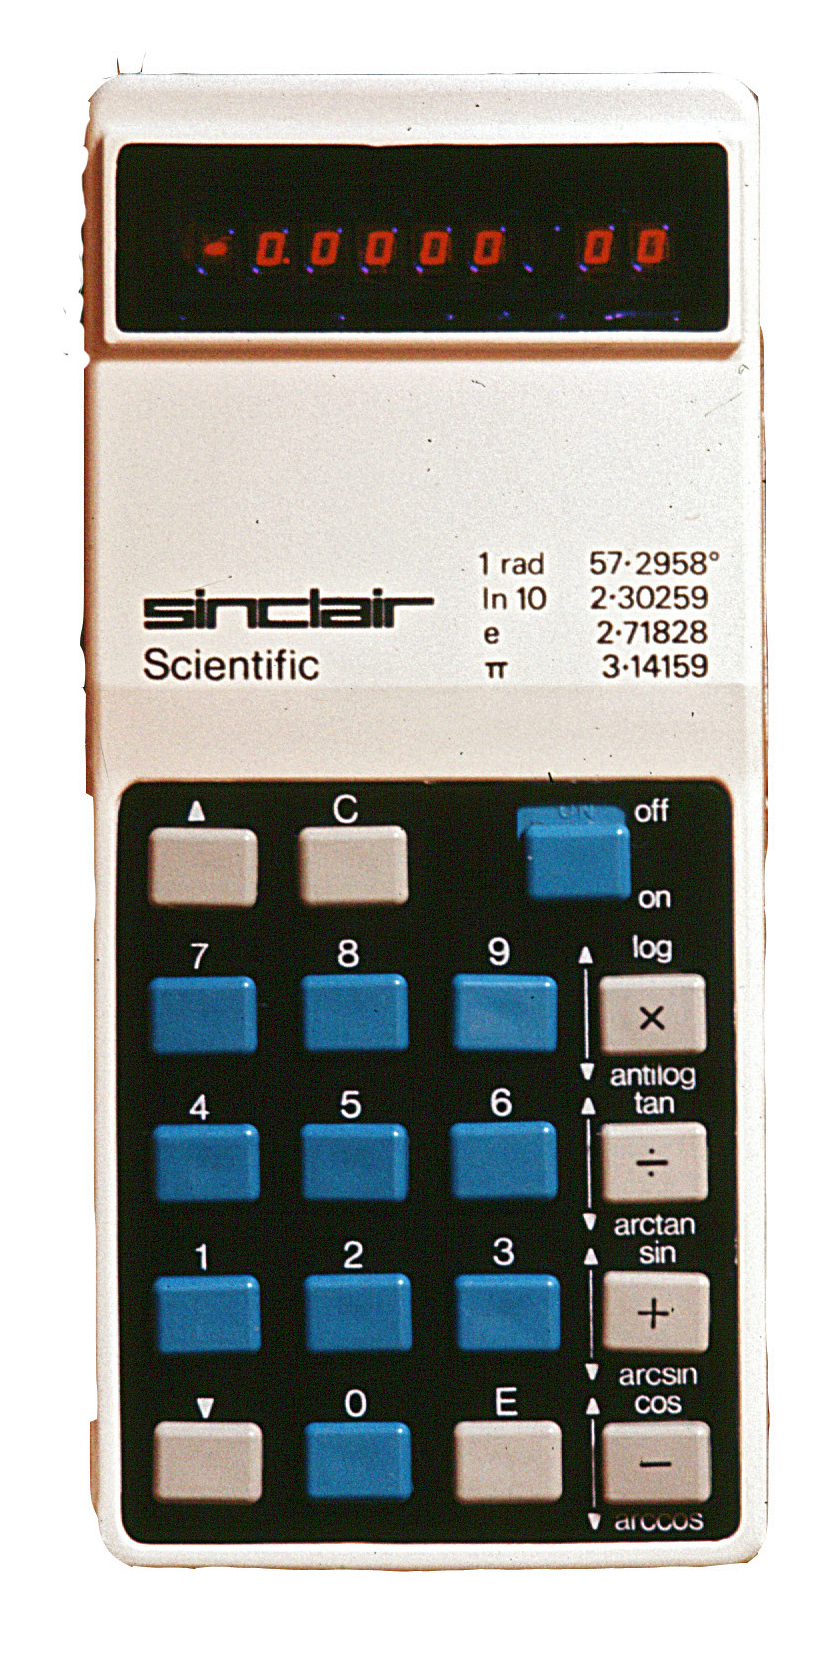
\includegraphics[height=\paperheight]{images/Sinclair_Scientific.jpg}}
\begin{frame}[plain]
\begin{columns}
  \column{0.4\textwidth}
  \column{0.6\textwidth}
  \begin{itemize}
    \item Welche Taste fehlt hier?
    \onslide<2>{
    \item Eingegebene Zahlen landen auf einem Stack
    \item $\times / \div / + / -$ wenden ihre Operation auf die obersten Stackelemente an
    \item Ergebnis landet wieder auf dem Stack
    \item Beispiel:\\
          $2 \times (7 + 14) \leadsto 2 \; 7 \; 14 + \times$
    \item \emph{Umgekehrte Polnische Notation}
    }
  \end{itemize}
  \vspace{1cm}
  {\small Sinclair Scientific (1974)}
\end{columns}
\end{frame}
}

\begin{frame}{UPN-Rechner}
  \code{../demos/rpn.pro}

  \begin{itemize}
    \item Beispiel: \texttt{eval([15, 27, plus], [42]).}
    \item Erweitert \texttt{evalOp} um $\times / \div / -$!
  \end{itemize}
\end{frame}

\begin{frame}{Übersetzung in UPN}
  \code{../demos/rpn2.pro}

  \begin{itemize}
    \item Vervollständigt \texttt{compile/2}!
    \item Beispiel:\\
          \texttt{compile(2 * (7 + 14), [2, 7, 14, plus, mul])}
  \end{itemize}
\end{frame}

\section{Haskell}

\begin{frame}{Pixelflut}
  Mit dem Pixelflut-Protokoll können wir einzelne Pixel per TCP auf eine Leinwand malen.
  Es gibt zwei einfache Befehle:

  \begin{itemize}
    \item \texttt{SIZE}: Fragt die Größe der Leinwand ab
    \item \texttt{PX x y rrggbb}: Zeichnet einen Pixel der Farbe \texttt{rrggbb}
  \end{itemize}

  Mit \texttt{nc} oder \texttt{telnet} könnt ihr euch mit meinem Pixelflut-Server verbinden:

  \begin{itemize}
    \item \texttt{nc XXX.XXX.XXX.XXX 3000}
    \item \texttt{telnet XXX.XXX.XXX.XXX:3000}
  \end{itemize}

  Verwendet die Vorlage in \texttt{demos/Pixelflut.hs} um per Haskell Pixel zu malen!
\end{frame}

\end{document}
